%        File: revise.tex
%     Created: Wed Jan 16 10:00 AM 2019 P
% Last Change: Wed Jan 16 10:00 AM 2019 P
%

%
% Copyright 2007, 2008, 2009 Elsevier Ltd
%
% This file is part of the 'Elsarticle Bundle'.
% ---------------------------------------------
%
% It may be distributed under the conditions of the LaTeX Project Public
% License, either version 1.2 of this license or (at your option) any
% later version.  The latest version of this license is in
%    http://www.latex-project.org/lppl.txt
% and version 1.2 or later is part of all distributions of LaTeX
% version 1999/12/01 or later.
%
% The list of all files belonging to the 'Elsarticle Bundle' is
% given in the file `manifest.txt'.
%

% Template article for Elsevier's document class `elsarticle'
% with numbered style bibliographic references
% SP 2008/03/01
%
%
%
% $Id: elsarticle-template-num.tex 4 2009-10-24 08:22:58Z rishi $
%
%
%\documentclass[preprint,12pt]{elsarticle}
\documentclass[answers,11pt]{exam}

% \documentclass[preprint,review,12pt]{elsarticle}

% Use the options 1p,twocolumn; 3p; 3p,twocolumn; 5p; or 5p,twocolumn
% for a journal layout:
% \documentclass[final,1p,times]{elsarticle}
% \documentclass[final,1p,times,twocolumn]{elsarticle}
% \documentclass[final,3p,times]{elsarticle}
% \documentclass[final,3p,times,twocolumn]{elsarticle}
% \documentclass[final,5p,times]{elsarticle}
% \documentclass[final,5p,times,twocolumn]{elsarticle}

% if you use PostScript figures in your article
% use the graphics package for simple commands
% \usepackage{graphics}
% or use the graphicx package for more complicated commands
\usepackage{graphicx}
% or use the epsfig package if you prefer to use the old commands
% \usepackage{epsfig}

% The amssymb package provides various useful mathematical symbols
\usepackage{amssymb}
% The amsthm package provides extended theorem environments
% \usepackage{amsthm}
\usepackage{amsmath}

% The lineno packages adds line numbers. Start line numbering with
% \begin{linenumbers}, end it with \end{linenumbers}. Or switch it on
% for the whole article with \linenumbers after \end{frontmatter}.
\usepackage{lineno}

% I like to be in control
\usepackage{placeins}

% natbib.sty is loaded by default. However, natbib options can be
% provided with \biboptions{...} command. Following options are
% valid:

%   round  -  round parentheses are used (default)
%   square -  square brackets are used   [option]
%   curly  -  curly braces are used      {option}
%   angle  -  angle brackets are used    <option>
%   semicolon  -  multiple citations separated by semi-colon
%   colon  - same as semicolon, an earlier confusion
%   comma  -  separated by comma
%   numbers-  selects numerical citations
%   super  -  numerical citations as superscripts
%   sort   -  sorts multiple citations according to order in ref. list
%   sort&compress   -  like sort, but also compresses numerical citations
%   compress - compresses without sorting
%
% \biboptions{comma,round}

% \biboptions{}


% Katy Huff addtions
\usepackage{xspace}
\usepackage{color}

\usepackage{multirow}
\usepackage[hyphens]{url}


\usepackage[acronym,toc]{glossaries}
%\newacronym{<++>}{<++>}{<++>}
\newacronym[longplural={metric tons of heavy metal}]{MTHM}{MTHM}{metric ton of heavy metal}
\newacronym{ABM}{ABM}{agent-based modeling}
\newacronym{ACDIS}{ACDIS}{Program in Arms Control \& Domestic and International Security}
\newacronym{ADS}{ADS}{Accelerator-Driven Systems}
\newacronym{AFCI}{AFCI}{Advanced Fuel Cycles Initiative}
\newacronym{AHTR}{AHTR}{Advanced High Temperature Reactor}
\newacronym{ANDRA}{ANDRA}{Agence Nationale pour la gestion des D\'echets RAdioactifs, the French National Agency for Radioactive Waste Management}
\newacronym{ANL}{ANL}{Argonne National Laboratory}
\newacronym{ANS}{ANS}{American Nuclear Society}
\newacronym{API}{API}{application programming interface}
\newacronym{ARE}{ARE}{Aircraft Reactor Experiment}
\newacronym{ARFC}{ARFC}{Advanced Reactors and Fuel Cycles}
\newacronym{ASME}{ASME}{American Society of Mechanical Engineers}
\newacronym{ASTRID}{ASTRID}{Advanced Sodium Technological Reactor for Industrial Demonstration}
\newacronym{ATWS}{ATWS}{Anticipated Transient Without Scram}
\newacronym{BDBE}{BDBE}{Beyond Design Basis Event}
\newacronym{BIDS}{BIDS}{Berkeley Institute for Data Science}
\newacronym{BWR}{BWR}{Boiling Water Reactor}
\newacronym{CAFCA}{CAFCA}{ Code for Advanced Fuel Cycles Assessment }
\newacronym{CDTN}{CDTN}{Centro de Desenvolvimento da Tecnologia Nuclear}
\newacronym{CEA}{CEA}{Commissariat \`a l'\'Energie Atomique et aux \'Energies Alternatives}
\newacronym{CI}{CI}{continuous integration}
\newacronym{CNEN}{CNEN}{Comiss\~{a}o Nacional de Energia Nuclear}
\newacronym{CNERG}{CNERG}{Computational Nuclear Engineering Research Group}
\newacronym{COSI}{COSI}{Commelini-Sicard}
\newacronym{COTS}{COTS}{commercial, off-the-shelf}
\newacronym{CSNF}{CSNF}{commercial spent nuclear fuel}
\newacronym{CTAH}{CTAHs}{Coiled Tube Air Heaters}
\newacronym{CUBIT}{CUBIT}{CUBIT Geometry and Mesh Generation Toolkit}
\newacronym{CURIE}{CURIE}{Centralized Used Fuel Resource for Information Exchange}
\newacronym{DAG}{DAG}{directed acyclic graph}
\newacronym{DANESS}{DANESS}{Dynamic Analysis of Nuclear Energy System Strategies}
\newacronym{DBE}{DBE}{Design Basis Event}
\newacronym{DESAE}{DESAE}{Dynamic Analysis of Nuclear Energy Systems Strategies}
\newacronym{DHS}{DHS}{Department of Homeland Security}
\newacronym{DOE}{DOE}{Department of Energy}
\newacronym{DRACS}{DRACS}{Direct Reactor Auxiliary Cooling System}
\newacronym{DRE}{DRE}{dynamic resource exchange}
\newacronym{DSNF}{DSNF}{DOE spent nuclear fuel}
\newacronym{DYMOND}{DYMOND}{Dynamic Model of Nuclear Development }
\newacronym{EBS}{EBS}{Engineered Barrier System}
\newacronym{EDF}{EDF}{Électricité de France}
\newacronym{EDZ}{EDZ}{Excavation Disturbed Zone}
\newacronym{EIA}{EIA}{U.S. Energy Information Administration}
\newacronym{EPA}{EPA}{Environmental Protection Agency}
\newacronym{EPR}{EPR}{European Pressurized Reactor}
\newacronym{EP}{EP}{Engineering Physics}
\newacronym{EU}{EU}{European Union}
\newacronym{FCO}{FCO}{Fuel Cycle Options}
\newacronym{FCT}{FCT}{Fuel Cycle Technology}
\newacronym{FEHM}{FEHM}{Finite Element Heat and Mass Transfer}
\newacronym{FEPs}{FEPs}{Features, Events, and Processes}
\newacronym{FHR}{FHR}{Fluoride-Salt-Cooled High-Temperature Reactor}
\newacronym{FLiBe}{FLiBe}{Fluoride-Lithium-Beryllium}
\newacronym{FP}{FP}{Fission Products}
\newacronym{GDSE}{GDSE}{Generic Disposal System Environment}
\newacronym{GDSM}{GDSM}{Generic Disposal System Model}
\newacronym{GENIUSv1}{GENIUSv1}{Global Evaluation of Nuclear Infrastructure Utilization Scenarios, Version 1}
\newacronym{GENIUSv2}{GENIUSv2}{Global Evaluation of Nuclear Infrastructure Utilization Scenarios, Version 2}
\newacronym{GENIUS}{GENIUS}{Global Evaluation of Nuclear Infrastructure Utilization Scenarios}
\newacronym{GPAM}{GPAM}{Generic Performance Assessment Model}
\newacronym{GRSAC}{GRSAC}{Graphite Reactor Severe Accident Code}
\newacronym{GUI}{GUI}{graphical user interface}
\newacronym{HLW}{HLW}{high level waste}
\newacronym{HPC}{HPC}{high-performance computing}
\newacronym{HTC}{HTC}{high-throughput computing}
\newacronym{HTGR}{HTGR}{High Temperature Gas-Cooled Reactor}
\newacronym{IAEA}{IAEA}{International Atomic Energy Agency}
\newacronym{IEMA}{IEMA}{Illinois Emergency Mangament Agency}
\newacronym{IHLRWM}{IHLRWM}{International High Level Radioactive Waste Management}
\newacronym{INL}{INL}{Idaho National Laboratory}
\newacronym{IPRR1}{IRP-R1}{Instituto de Pesquisas Radioativas Reator 1}
\newacronym{IRP}{IRP}{Integrated Research Project}
\newacronym{ISFSI}{ISFSI}{Independent Spent Fuel Storage Installation}
\newacronym{ISRG}{ISRG}{Independent Student Research Group}
\newacronym{JFNK}{JFNK}{Jacobian-Free Newton Krylov}
\newacronym{LANL}{LANL}{Los Alamos National Laboratory}
\newacronym{LBNL}{LBNL}{Lawrence Berkeley National Laboratory}
\newacronym{LCOE}{LCOE}{levelized cost of electricity}
\newacronym{LDRD}{LDRD}{laboratory directed research and development}
\newacronym{LFR}{LFR}{Lead-Cooled Fast Reactor}
\newacronym{LLNL}{LLNL}{Lawrence Livermore National Laboratory}
\newacronym{LMFBR}{LMFBR}{Liquid Metal Fast Breeder Reactor}
\newacronym{LOFC}{LOFC}{Loss of Forced Cooling}
\newacronym{LOHS}{LOHS}{Loss of Heat Sink}
\newacronym{LOLA}{LOLA}{Loss of Large Area}
\newacronym{LP}{LP}{linear program}
\newacronym{LWR}{LWR}{Light Water Reactor}
\newacronym{MAGNOX}{MAGNOX}{Magnesium Alloy Graphie Moderated Gas Cooled Uranium Oxide Reactor}
\newacronym{MA}{MA}{minor actinide}
\newacronym{MCNP}{MCNP}{Monte Carlo N-Particle code}
\newacronym{MILP}{MILP}{mixed-integer linear program}
\newacronym{MIT}{MIT}{the Massachusetts Institute of Technology}
\newacronym{MOAB}{MOAB}{Mesh-Oriented datABase}
\newacronym{MOOSE}{MOOSE}{Multiphysics Object-Oriented Simulation Environment}
\newacronym{MOX}{MOX}{Mixed Oxide Fuel}
\newacronym{MSBR}{MSBR}{Molten Salt Breeder Reactor}
\newacronym{MSRE}{MSRE}{Molten Salt Reactor Experiment}
\newacronym{MSR}{MSR}{Molten Salt Reactor}
\newacronym{MWe}{MWe}{Megawatts electric}
\newacronym{NAGRA}{NAGRA}{National Cooperative for the Disposal of Radioactive Waste}
\newacronym{NEAMS}{NEAMS}{Nuclear Engineering Advanced Modeling and Simulation}
\newacronym{NEUP}{NEUP}{Nuclear Energy University Programs}
\newacronym{NFCSim}{NFCSim}{Nuclear Fuel Cycle Simulator}
\newacronym{NGNP}{NGNP}{Next Generation Nuclear Plant}
\newacronym{NMWPC}{NMWPC}{Nuclear MW Per Capita}
\newacronym{NNSA}{NNSA}{National Nuclear Security Administration}
\newacronym{NPRE}{NPRE}{Department of Nuclear, Plasma, and Radiological Engineering}
\newacronym{NQA1}{NQA-1}{Nuclear Quality Assurance - 1}
\newacronym{NRC}{NRC}{Nuclear Regulatory Commission}
\newacronym{NSF}{NSF}{National Science Foundation}
\newacronym{NSSC}{NSSC}{Nuclear Science and Security Consortium}
\newacronym{NUWASTE}{NUWASTE}{Nuclear Waste Assessment System for Technical Evaluation}
\newacronym{NWF}{NWF}{Nuclear Waste Fund}
\newacronym{NWTRB}{NWTRB}{Nuclear Waste Technical Review Board}
\newacronym{OCRWM}{OCRWM}{Office of Civilian Radioactive Waste Management}
\newacronym{ORION}{ORION}{ORION}
\newacronym{ORNL}{ORNL}{Oak Ridge National Laboratory}
\newacronym{PARCS}{PARCS}{Purdue Advanced Reactor Core Simulator}
\newacronym{PBAHTR}{PB-AHTR}{Pebble Bed Advanced High Temperature Reactor}
\newacronym{PBFHR}{PB-FHR}{Pebble-Bed Fluoride-Salt-Cooled High-Temperature Reactor}
\newacronym{PEI}{PEI}{Peak Environmental Impact}
\newacronym{PHWR}{Pressurized Heavy Water Reactor}{Pressurized Heavy Water Reactor}
\newacronym{PH}{PRONGHORN}{PRONGHORN}
\newacronym{PRIS}{PRIS}{Power Reactor Information System}
\newacronym{PRKE}{PRKE}{Point Reactor Kinetics Equations}
\newacronym{PSPG}{PSPG}{Pressure-Stabilizing/Petrov-Galerkin}
\newacronym{PWAR}{PWAR}{Pratt and Whitney Aircraft Reactor}
\newacronym{PWR}{PWR}{Pressurized Water Reactor}
\newacronym{PyNE}{PyNE}{Python toolkit for Nuclear Engineering}
\newacronym{PyRK}{PyRK}{Python for Reactor Kinetics}
\newacronym{QA}{QA}{quality assurance}
\newacronym{RDD}{RD\&D}{Research Development and Demonstration}
\newacronym{RD}{R\&D}{Research and Development}
\newacronym{RELAP}{RELAP}{Reactor Excursion and Leak Analysis Program}
\newacronym{RIA}{RIA}{Reactivity Insertion Accident}
\newacronym{RIF}{RIF}{Region-Institution-Facility}
\newacronym{SFR}{SFR}{Sodium-Cooled Fast Reactor}
\newacronym{SINDAG}{SINDA{\textbackslash}G}{Systems Improved Numerical Differencing Analyzer $\backslash$ Gaski}
\newacronym{SKB}{SKB}{Svensk K\"{a}rnbr\"{a}nslehantering AB}
\newacronym{SNF}{SNF}{spent nuclear fuel}
\newacronym{SNL}{SNL}{Sandia National Laboratory}
\newacronym{STC}{STC}{specific temperature change}
\newacronym{SUPG}{SUPG}{Streamline-Upwind/Petrov-Galerkin}
\newacronym{SWF}{SWF}{Separations and Waste Forms}
\newacronym{SWU}{SWU}{Separative Work Unit}
\newacronym{TRIGA}{TRIGA}{Training Research Isotope General Atomic}
\newacronym{TRISO}{TRISO}{Tristructural Isotropic}
\newacronym{TSM}{TSM}{Total System Model}
\newacronym{TSPA}{TSPA}{Total System Performance Assessment for the Yucca Mountain License Application}
\newacronym{ThOX}{ThOX}{thorium oxide}
\newacronym{UFD}{UFD}{Used Fuel Disposition}
\newacronym{UML}{UML}{Unified Modeling Language}
\newacronym{UNF}{UNF}{Used Nuclear Fuel}
\newacronym{UOX}{UOX}{Uranium Oxide Fuel}
\newacronym{UQ}{UQ}{uncertainty quantification}
\newacronym{US}{US}{United States}
\newacronym{UW}{UW}{University of Wisconsin}
\newacronym{VISION}{VISION}{the Verifiable Fuel Cycle Simulation Model}
\newacronym{VVER}{VVER}{Voda-Vodyanoi Energetichesky Reaktor (Russian Pressurized Water Reactor)}
\newacronym{VV}{V\&V}{verification and validation}
\newacronym{WIPP}{WIPP}{Waste Isolation Pilot Plant}
\newacronym{YMR}{YMR}{Yucca Mountain Repository Site}


\makeglossaries

%\journal{Annals of Nuclear Energy}

\begin{document}

%\begin{frontmatter}

% Title, authors and addresses

% use the tnoteref command within \title for footnotes;
% use the tnotetext command for the associated footnote;
% use the fnref command within \author or \address for footnotes;
% use the fntext command for the associated footnote;
% use the corref command within \author for corresponding author footnotes;
% use the cortext command for the associated footnote;
% use the ead command for the email address,
% and the form \ead[url] for the home page:
%
% \title{Title\tnoteref{label1}}
% \tnotetext[label1]{}
% \author{Name\corref{cor1}\fnref{label2}}
% \ead{email address}
% \ead[url]{home page}
% \fntext[label2]{}
% \cortext[cor1]{}
% \address{Address\fnref{label3}}
% \fntext[label3]{}

\title{Synergistic Spent Nuclear Fuel Dynamics Within the European Union\\
        \large Response to Review Comments}
\author{Jin Whan Bae, Clifford E. Singer, Kathryn D. Huff}

% use optional labels to link authors explicitly to addresses:
% \author[label1,label2]{<author name>}
% \address[label1]{<address>}
% \address[label2]{<address>}


%\author[uiuc]{Kathryn Huff}
%        \ead{kdhuff@illinois.edu}
%  \address[uiuc]{Department of Nuclear, Plasma, and Radiological Engineering,
%        118 Talbot Laboratory, MC 234, Universicy of Illinois at
%        Urbana-Champaign, Urbana, IL 61801}
%
% \end{frontmatter}
\maketitle
\section*{Review General Response}
We would like to thank the reviewers for their detailed assessment of
this paper. Your comments have resulted in changes which certainly improved the 
paper. We have re-run the many simulations in this paper according to the 
suggestions in this work and the results have been updated.


\section*{Reviewer 1}
\begin{questions}
    \question In Table 4 the BWR initial enrichment is now given as 5.8 w/o which seems high to me. Not only does this not match the mean discharge burnup, but it exceeds the 5.0 w/o criticality limit in current fuel fabrication plants. 

    \begin{solution}
    Thank you for your insight. The $5.8 ^{235}U$ value in table 4
    is the initial fissile loading in tonnes. Given the core size
    ($~137$ tonnes), the enrichment is therefore $4.2\%$.
    \end{solution}


    \question I don't understand Figure 9 - there is a blue line captioned "from reprocessed LWR UNF", but the line is hardly showing in the graph. Is this intended?

    \begin{solution}
    The blue line is supposed to be a very thin plane. We intentionally
    plotted this to show that the ASTRID fuel that can be created
    from outstanding French \gls{LWR} \gls{UNF} is very small.
    \end{solution}

    \question Very trivial: Table 12 footnote should read "... are not considered for ..."

    \begin{solution}
        Thank you. We made sure the table 12 footnote says `` are not considered for ''
    \end{solution}


\end{questions}
\section*{Reviewer 2}
\begin{questions}
    \question First, the authors refer to the ASTRID reactors as becoming "independent"; I think a more clear term here would be "self-sustaining" in that this fleet is exclusively relying upon plutonium bred from this fleet to sustain core reloadings. (Note that I understand the authors' intent; effectively the ASTRID fleet decouples from the LWR fleet, but it may simply make this point more clearly.)

    \begin{solution}
    That is a very good point, thank you. We have made the changes
    accordingly.
    \end{solution}

    \question Second, in Table 11, I assume the authors mean "Average LWR UNF reprocessed (PER MONTH)" and "(Total) Average UNF reprocessed (PER MONTH)". (Alternatively, these might be expressed as, "Average monthly LWR UNF reprocessing demand" and "Average monthly total UNF reprocessing demand"). I point this out because this can become a bit confusing; the first two entries on this table correspond to absolute values of mass (MT UNF / ASTRID fuel), whereas the second two correspond to RATES (fuel processing demand). The authors make this clear in the text, but I had to go through and re-read after looking at the table to grasp this subtle difference.

    \begin{solution}
    That is a very good point. We made the following changes
    in table 11 for clarity:
    
    Average LWR UNF reprocessed $\rightarrow$ Avg. LWR UNF reprocessed [per month]

    Average UNF reprocessed $\rightarrow$ Avg. UNF reprocessed [per month]

    \end{solution}

    \question Additionally, while a comparison of the average reprocessing
    demand resulting from LWR life extensions is useful, one other
     feature I observed is in the peak reprocessing demand (which roughly appears to correlate 
     with the LWR phase-out period and second phase of ASTRID construction). Essentially,
    it would appear that the peak monthly reprocessing demand is just over 40 MTHM/month,
    whereas the average demand is well under 30 MTHM. Effectively then, the reprocessing 
    capacity specified in Table 3 doesn't seem to be limiting (unless I am mistaken). The
    authors appear to assume a doubling of reprocessing capacity post-ASTRID, but this 
    assumption doesn't seem to be required or justified by the physics; if anything,
    maintaining (or even drawing down) capacity would seem to be in order. I don't think
    the authors should go back and repeat the study for this, but it is certainly a
    policy-relevant outcome worth noting.

    \begin{solution}
        If you are looking at Figure 14 for the reprocessing demand, the figure
        represents the amount of plutonium discharged from the reprocessing plants,
        which is proportional to the amount of \gls{UNF} reprocessed. To get the
        reprocessing demand, one should multiply the `pu from legacy' value by
        approximately 100 (since plutonium is \textasciitilde 1\% of \gls{LWR} \gls{UNF})
        and the `pu from spent sfr fuel' by 4.17 (plutonium is \textasciitilde 24\% of
        ASTRID \gls{UNF}). So the average reprocessing demand would be closer to
        125.1 MTHM /month, with a peak reprocessing demand being around 166.8 MTHM / month.

        Another thing to note is that the plutonium outflux from the reprocessing facilities
        does not directly reflect the plutonium demand for ASTRID fuels. The best way to 
        predict reprocessing demand is to look at actual ASTRID fuel demand and `back calculate'
        the \gls{UNF} reprocessing demand. We understand that this is not clear in the paper,
        so we added a plot showing the average reprocessing demand.

        \centering
        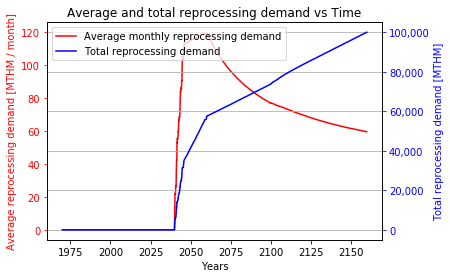
\includegraphics[width=0.7\textwidth]{../images/french-transition/avg_tot_rep.png}

    \end{solution}

    \question Finally, while I know it's nitpicky, you may want to reference the equation on Page 25 by a LaTeX label, rather than relative physical position.

    \begin{solution}
    You are absolutely right. We have made changes accordingly.
    Thank you.
    \end{solution}

    \question Otherwise, I greatly appreciate the effort the authors have put in to clarify working assumptions used in this work,
    particularly as they pertain to both assumptions used to calculate the depleted fuel recipe as well as assumptions (and the limitations thereof)
    for the fuel vector supplied to the ASTRID fleet. Some of these assumptions, such as the breeding ratio,
    while ignoring practical operational considerations are nonetheless instructive as an high-level sensitivity analysis.
    The additions that the authors have made to caveat and bound these assumptions is quite helpful.

    \begin{solution}
    Thank you for your kindness. We believe that you and the other reviewers' comments greatly enriched
    this paper as a whole. Thank you.
    \end{solution}






\end{questions}
%\bibliographystyle{unsrt}
%\bibliography{revise}
\end{document}

  %
  % End of file `elsarticle-template-num.tex'.
